\chapter{Additional results}
\chref{results_extra}

\section{Action log results}
\subsection{Correlations}
From the data gathered from the log files, it is interesting to see if there is any correlation between the rating of the outcome and any other parameter. \Figref{graph_correlation} shows four presumed possible correlations, with data points for both the naive and the smart version of \oframp. Trend lines have been plotted - a cyan one for the naive version and a magenta line for the smart - to help identifying if there is any correlation.

\begin{figure}[h!]
\centering
\begin{subfigure}[t]{0.48\textwidth}
\centering
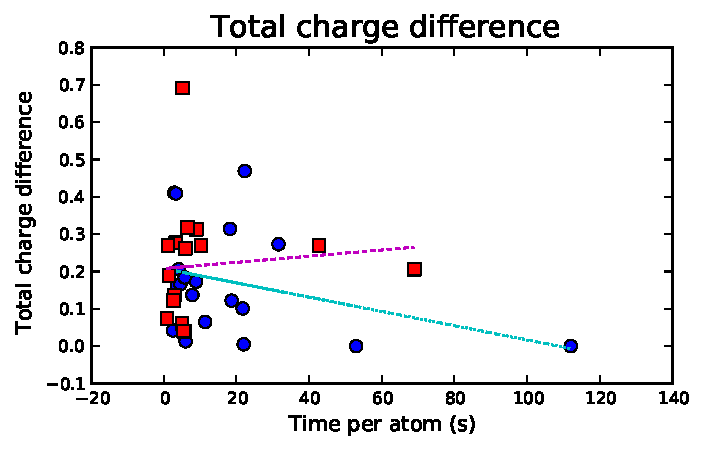
\includegraphics[width=\textwidth]{img/graphs/3a_01.pdf}
\caption{Total charge difference in relation to the average time used per atom.}
\figlab{graph_correlation_1}
\end{subfigure}%
~
\begin{subfigure}[t]{0.48\textwidth}
\centering
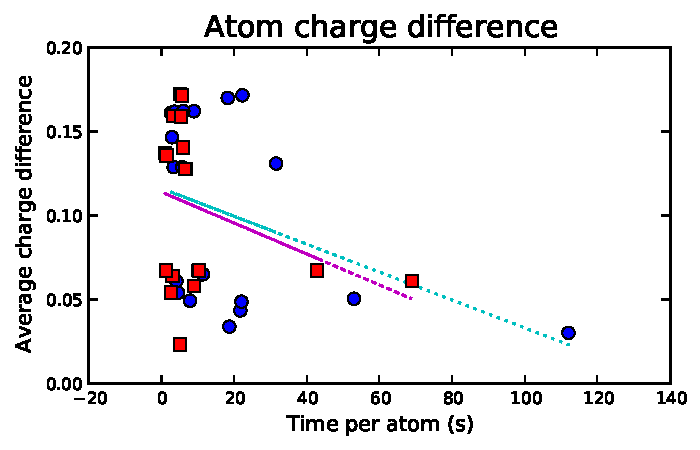
\includegraphics[width=\textwidth]{img/graphs/3a_00.pdf}
\caption{Average charge difference per atom in relation to the average time used per atom.}
\figlab{graph_correlation_2}
\end{subfigure}%
\\[1em]
\begin{subfigure}[t]{0.48\textwidth}
\centering
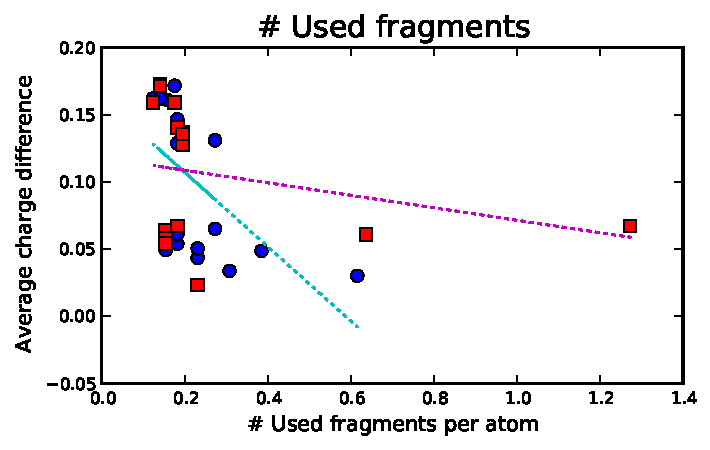
\includegraphics[width=\textwidth]{img/graphs/3a_02.pdf}
\caption{Average charge difference per atom in relation to the number of used fragments per atom.}
\figlab{graph_correlation_3}
\end{subfigure}%
~
\begin{subfigure}[t]{0.48\textwidth}
\centering
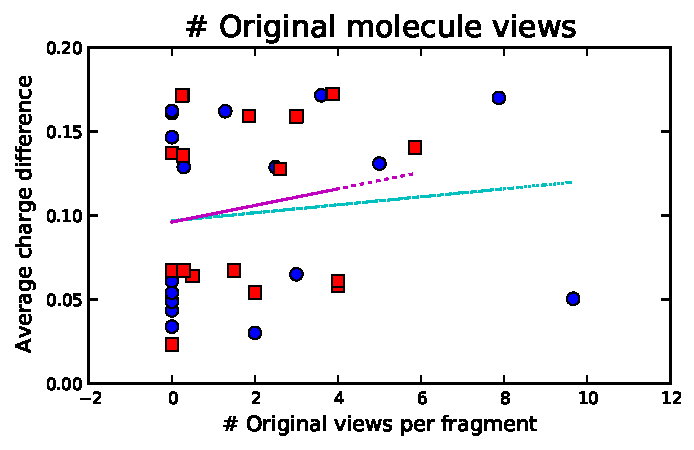
\includegraphics[width=\textwidth]{img/graphs/3a_03.pdf}
\caption{Average charge difference per atom in relation to the number of original molecule views per selected fragment.}
\figlab{graph_correlation_4}
\end{subfigure}
\caption{Presumed correlations between user studies outcomes. The blue circles are data points gathered from the naive version, the red squares come from the smart version.}
\figlab{graph_correlation}
\end{figure}

However, as one can see almost immediately, there does not appear to be any correlation between any of the graphs shown in \figref{graph_correlation}. Even when the most extreme outliers are removed, the data points are still widely scattered and no correlation can be observed.

When taking a look at \figref{graph_correlation_1} and \figref{graph_correlation_2}, it does appear that the parameterisations the most time has been spent on are amongst the best rated. However, they are not \emph{the} best rated, and may just be outliers as they are found in isolation from the rest of the points. Furthermore, for the smart version, the users that spent the most time are not performing better than average, but these may still be outliers. A larger test group would be needed to confirm the (lack of) correlation here.

Just like is the case for the charge differences, the extremes in the number of used fragments are among the best results~(see \figref{graph_correlation_3}). However, it may also be the case here that these points are just outliers, and more experimentation is needed to be able to observe any real trend.

For the number of original molecule views, the results are the most widespread~(see \figref{graph_correlation_4}). It appears that viewing many original molecules has absolutely no effect on the quality of the parameterisation result. Furthermore, the best results for both the naive and smart version of \oframp{} are obtained by users who did not check a single original molecule. This is an interesting observation, as it is believed that, in order to judge if a fragment is a good match, one needs to see the fragment in the context of its originating molecule.